\section{Feasibility Study}

Below we show how it's possible to directly implement the three main vector type transformations (along
with a couple of other particularly useful ones) in Idris, which are guaranteed to be correct at compile time.

The \textit{Shape} of a vector is defined as an Idris \textit{Vect} of a given number dimensions, each
represented as a natural number. This shape is used to define the vector type.

Defining the vector requires a recursive type definition, having the base case of a 0 dimensional vector 
equivalent to the base vector type. This follows from the result that if any dimension in the
vector has 0 elements, then the vector itself must have no elements.

\inputIdrisListing{code/vector.idr}


\subsection{Implementing Vector Type Transformation Functions}

From the \textit{Vector} definition it's trivial to define the \textit{singleton} function
as a function taking an n dimensional \textit{Vector} and mapping it to a 1+n dimensional
\textit{Vector}, as well as its inverse function:

\inputIdrisListing{code/singleton.idr}


Defining the \textit{map} instance uses pattern matching on the dependent types
to check whether the number of dimensions the \textit{Vector} has is 0, in which case the 
given function is applied to the single element. Otherwise the map function is applied
recursively to all elements in the \textit{Vector} until all the base elements have been
transformed.

\inputIdrisListing{code/map.idr}


Taking a given \textit{Vector} which has 2 or more dimensions, we can decrease 
the dimensionality by 1 by concatenating all the Sub-Vectors as follows
\inputIdrisListing{code/redDim.idr}
This results in a \textit{Vector} with a dimensionality of one less than the input \textit{Vector}.
The new \textit{Vector} contains the same elements as the input \textit{Vector}, and ordering is
also preserved. 


\begin{figure*}
\begin{center}
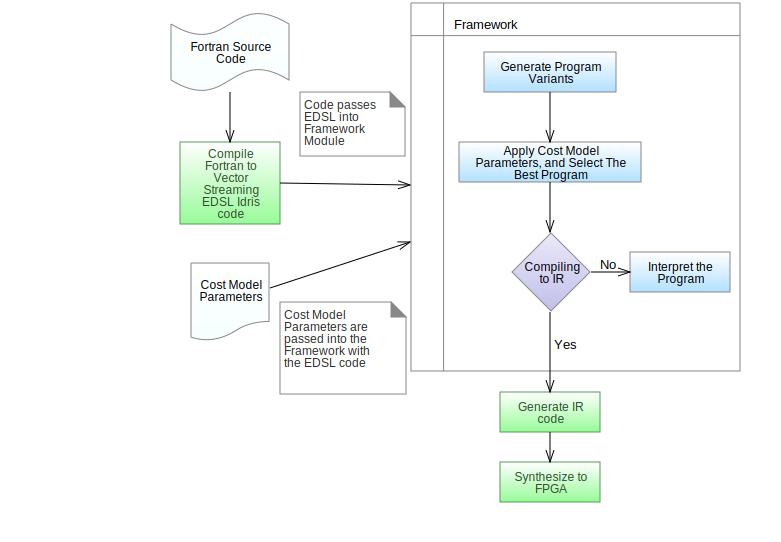
\includegraphics[scale=0.65]{images/flow.pdf}
\caption{Flowchart illustrating the structure of the Framework.}
\label{flow}
\end{center}
\end{figure*}

\inputIdrisListing{code/reshape.idr}
\newpage
\inputIdrisListing{code/reshapeInv.idr}


Taking a given \textit{Vector} which has 1 or more dimensions; in which the most "outer" dimension is
made up of \textbf{n * m} elements, where \textbf{n, m} $\in \mathbb{N}$. We can increase the dimensionality of
the given \textit{Vector} by 1 by splitting the \textit{Vector} at each \textbf{n} sub-Vectors which results in 
\textbf{m} lots of \textbf{n} sub-Vectors. 
\inputIdrisListing{code/incDim.idr}


Defining the \textit{reshape} transformation function and its inverse can be achieved with aid from the 
increase and decreasing dimensional transformations listed above.


Due to Idris' support for implementing EDSLs, and the ability to directly implement
the vector transformations, it should be feasible to fit these transformations
into an EDSL. 


